% Tikz File 'mytikz.tex'
\documentclass{standalone}
\input{../Mod_base/grafica}

%\usetikzlibrary{...}
\begin{document}
	

		\begin{tikzpicture}[cap=round,>=latex,scale=5.3]
		% draw the coordinates
		\draw[->] (-1.5cm,0cm) -- (1.5cm,0cm) node[right,fill=white] {$x$};
		\draw[->] (0cm,-1.5cm) -- (0cm,1.5cm) node[above,fill=white] {$y$};
		
		% draw the unit circle
		\draw[thick] (0cm,0cm) circle(1cm);
		
		\foreach \x in {0,30,...,360} {
			% lines from center to point
			\draw[gray] (0cm,0cm) -- (\x:1cm);
			% dots at each point
			\filldraw[black] (\x:1cm) circle(0.4pt);
			% draw each angle in degrees
			\draw (\x:0.6cm) node[fill=white] {$\x^\circ$};
		}
		% draw each angle in radians
		\foreach \x/\xtext in {
			30/\dfrac{\pi}{6},
			45/\dfrac{\pi}{4},
			60/\dfrac{\pi}{3},
			90/\dfrac{\pi}{2},
			120/\dfrac{2\pi}{3},
			135/\dfrac{3\pi}{4},
			150/\dfrac{5\pi}{6},
			180/\pi,
			210/\dfrac{7\pi}{6},
			225/\dfrac{5\pi}{4},
			240/\dfrac{4\pi}{3},
			270/\dfrac{3\pi}{2},
			300/\dfrac{5\pi}{3},
			315/\dfrac{7\pi}{4},
			330/\dfrac{11\pi}{6},
			360/2\pi}
		\draw (\x:0.85cm) node[fill=white] {$\xtext$};
		
		\foreach \x/\xtext/\y in {
			% the coordinates for the first quadrant
			30/\dfrac{\sqrt{3}}{2}/\dfrac{1}{2},
			45/\dfrac{\sqrt{2}}{2}/\dfrac{\sqrt{2}}{2},
			60/\dfrac{1}{2}/\dfrac{\sqrt{3}}{2},
			% the coordinates for the second quadrant
			150/-\dfrac{\sqrt{3}}{2}/\dfrac{1}{2},
			135/-\dfrac{\sqrt{2}}{2}/\dfrac{\sqrt{2}}{2},
			120/-\dfrac{1}{2}/\dfrac{\sqrt{3}}{2},
			% the coordinates for the third quadrant
			210/-\dfrac{\sqrt{3}}{2}/-\dfrac{1}{2},
			225/-\dfrac{\sqrt{2}}{2}/-\dfrac{\sqrt{2}}{2},
			240/-\dfrac{1}{2}/-\dfrac{\sqrt{3}}{2},
			% the coordinates for the fourth quadrant
			330/\dfrac{\sqrt{3}}{2}/-\dfrac{1}{2},
			315/\dfrac{\sqrt{2}}{2}/-\dfrac{\sqrt{2}}{2},
			300/\dfrac{1}{2}/-\dfrac{\sqrt{3}}{2}}
		\draw (\x:1.25cm) node[fill=white] {$\left(\xtext,\y\right)$};
		
		% draw the horizontal and vertical coordinates
		% the placement is better this way
		\draw (-1.25cm,0cm) node[above=1pt] {$(-1,0)$}
		(1.25cm,0cm)  node[above=1pt] {$(1,0)$}
		(0cm,-1.25cm) node[fill=white] {$(0,-1)$}
		(0cm,1.25cm)  node[fill=white] {$(0,1)$};
		\end{tikzpicture}
\end{document}